\newcommand{\sur}[1]{\ensuremath{^{\textrm{#1}}}}
\newcommand{\sous}[1]{\ensuremath{_{\textrm{#1}}}}
\newenvironment{Snugshade}[1][236,236,236]{
  \definecolor{shadecolor}{RGB}{#1}%
  \begin{snugshade}%
}{%
    \end{snugshade}%
}
\definecolor{shadecolor}{RGB}{236,236,236} %defines color of snugshade box
\section{Overview}


This tutorial presents the general principles of assessing the reliability of a phylogenetic inference through the use
of posterior predictive simulation (PPS). PPS works by assessing the fit of an evolutionary model to a given dataset,
and analyzing several test statistics using a traditional goodness-of-fit framework to help explain where a model
may be the most inadequate. 

\subsection{Requirements}
We assume that you have read and hopefully completed the following tutorials:
\begin{itemize}
\item RB\_Getting\_Started
\item RB\_Data\_Tutorial
\item RB\_MCMC\_Tutorial
\end{itemize}
This means that we will assume that you know how to execute and load data into \RevBayes, are familiar 
with some basic commands, and know how to perform an analysis of a single-gene dataset (assuming an 
unconstrained/unrooted tree).


%%%%%%%%
%%   Data   %%
%%%%%%%%
\section{Data and files}

We provide the necessary data and scripts that we will use in this tutorial.
Of course, you may want to use your own dataset instead.
In the \cl{data} folder, you will find the following files
\begin{itemize}
\item \textbf{data/primates\_and\_galeopterus\_cytb.nex}: A simple dataset consisting of 8 taxa with 500 characters simulated under the GTR model.
\end{itemize}

\section{Specific Style Notes For This Tutorial}
Throughout this tutorial you will see code snippets in various boxes like this: 
{\tt \begin{snugshade*}
\begin{lstlisting}
CODE SNIPPET IN FILE
\end{lstlisting}
\end{snugshade*}}

if the snippet is in a grey box like the one above, that is code you should inspect or tweak in a \textbf{.Rev} file.
If the code is in blue like this: 
{\tt \begin{Snugshade}[184,207,236]
\begin{lstlisting}
CODE SNIPPET TO TYPE DIRECTLY INTO RevBayes
\end{lstlisting}
\end{Snugshade}}
you should type this code directly into the \RevBayes prompt in your terminal window.

\section{Introduction}
Assessing the fit of an evolutionary model to the data is critical as using a model with poor fit can lead to 
spurious conclusions. However, a critical evaluation of absolute model fit is rare in evolutionary studies.
Posterior prediction is a Bayesian approach to assess the fit of a model to a given dataset \citep{Bollback2002-ki,Brown2014-jl,Gelman2014-ay},
that relies on the use of the posterior and the posterior predictive distributions. 
The posterior distribution is the standard output from Bayeisan phylogenetic inference. The posterior predictive 
distribution represents a range of possible outcomes given the assumptions of the model. The most common method to 
generate these possible outcomes, is to sample parameters from the posterior distribution, and use them 
to simulate new replicate datasets (Fig. 1). If these simulated datasets differ from the empirical dataset in a
meaningful way, the model is failing to capture some salient feature of the evolutionary process. 

\begin{figure}[h!]
\centering
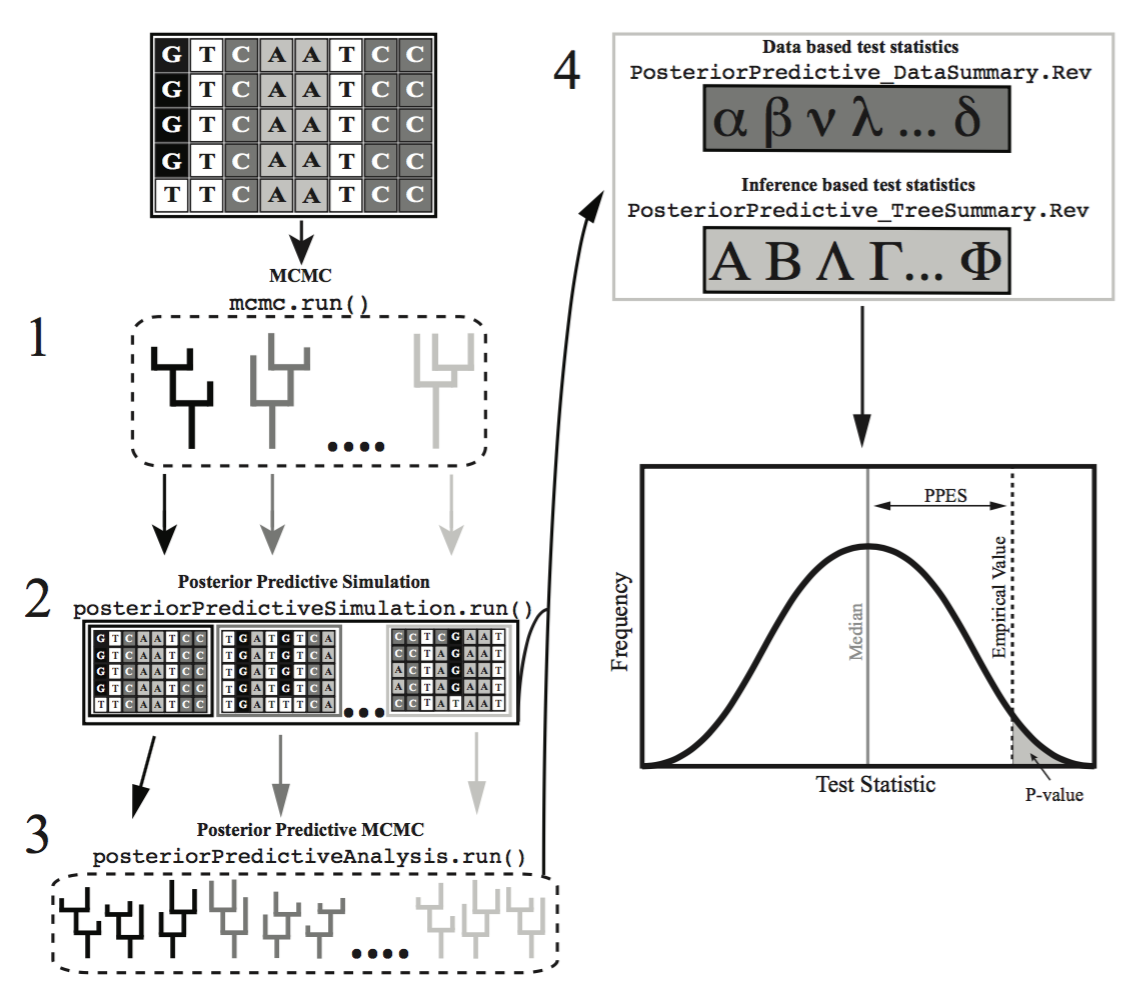
\includegraphics[width=\textwidth,angle=0]{figures/pps.png}
\caption{\small A cartoon schematic showing the process of assessing model fit with posterior predictive simulation built into P\sur{3} and \RevBayes. \label{"Figure 1"}}
\end{figure}
\end{centering}
The framework to construct posterior predictive distributions, and compare them to the posterior distribution is 
conveniently built in to \RevBayes. In this tutorial we will walk you through using this functionality to perform
a complete posterior predictive simulation on an example dataset.  


\bigskip
\subsection{Substitution Models}\label{secUnif} 

The models we use here are equivalent to the models described in the previous exercise on substitution models (continuous time Markov models).
To specify the model please consult the previous exercise. Specifically, you will need to specify the following substitution models:
\begin{itemize}
\item Jukes-Cantor (JC) substitution model \citep{Jukes1969-jp}
\item General-Time-Reversible (GTR) substitution model \citep{Tavare1986-ij}
\item Gamma (+G) model for among-site rate variation \citep{Yang1994-ep}
\item Invariable-sites (+I) model \citep{Hasegawa1985-ir}
\end{itemize}


\bigskip
\section{Assessing Model Fit with Posterior Prediction}

The entire process of posterior prediction can be executed by using the \textbf{full\_analysis.Rev} script in the \textbf{scripts}
folder. If you were to type the following command into \RevBayes:

{\tt \begin{snugshade*}
\begin{lstlisting}
source("scripts/full_analysis_JC.Rev")
\end{lstlisting}
\end{snugshade*}}

the entire posterior prediction process would run on the example dataset. However, in this tutorial, we 
will walk through each step of this process on an example dataset. 

\subsection{Empirical MCMC Analysis}

To begin, we first need to generate a posterior distribution from which to sample for simulation. 
This is the normal, and often only, step conducted in phylogenetic studies. Here we will specify our 
dataset, evolutionary model, and run a traditional MCMC analysis. 

In the the \textbf{full\_analysis\_JC.Rev} script, this step is conducted with the following lines of RevScript:

{\tt \begin{snugshade*}
\begin{lstlisting}
## EMPIRICAL MCMC
inFile = "data/primates_and_galeopterus_cytb.nex"
analysis_name = "pps_example"
data <- readDiscreteCharacterData(inFile)
model_name = "JC"
model_file_name = "scripts/"+model_name+"_Model.Rev"
source("scripts/MCMC_Simulation.Rev")
\end{lstlisting}
\end{snugshade*}}

Let's break down each of these lines and the scripts they call in order to better understand what is 
happening. 

{\tt \begin{snugshade*}
\begin{lstlisting}
inFile = "data/primates_and_galeopterus_cytb.nex"
\end{lstlisting}
\end{snugshade*}}

This line is just specifying an input file name. This is your data, in NEXUS format.

{\tt \begin{snugshade*}
\begin{lstlisting}
analysis_name = "pps_example"
\end{lstlisting}
\end{snugshade*}}

This line is just specifying a general name to apply to your analysis. This will be used for future output files, so make sure it's something clear and easy to understand.

{\tt \begin{snugshade*}
\begin{lstlisting}
data <- readDiscreteCharacterData(inFile)
\end{lstlisting}
\end{snugshade*}}

This line reads in the data file into a data object in \RevBayes. 

 
{\tt \begin{snugshade*}
\begin{lstlisting}
model_name = "JC"
model_file_name = "scripts/"+model_name+"_Model.Rev"
\end{lstlisting}
\end{snugshade*}}

Here we are specifying an evolutionary substitution model to use with the MCMC analysis. In this specific
case, we are using the Jukes-Cantor (JC) model for this example. If we open the \textbf{JC\_Model.Rev} 
script, most of this script should look familiar from the \item RB\_MCMC\_Tutorial. There are a couple of specific 
lines we can look at that might be a little different though, as we are using a unrooted tree for this
analysis. 

{\tt \begin{snugshade*}
\begin{lstlisting}
Q <-fnJC(4)
\end{lstlisting}
\end{snugshade*}}

Here we are specifying that we should use the Jukes-Cantor model, and have it applied uniformly to all sites in 
the dataset. While this obviously is not likely to be a good fitting model for most datasets, we are using it for 
simplicity of illustrating the process. 

{\tt \begin{snugshade*}
\begin{lstlisting}
topology ~ dnUniformTopology(names)
\end{lstlisting}
\end{snugshade*}}
This sets a uniform prior on the tree topology.
{\tt \begin{snugshade*}
\begin{lstlisting}
br_lens[i] ~ dnExponential(10.0)
\end{lstlisting}
\end{snugshade*}}
This sets an exponential distribution as the branch length prior.
{\tt \begin{snugshade*}
\begin{lstlisting}
phylogeny := treeAssembly(topology, br_lens)
\end{lstlisting}
\end{snugshade*}}
This builds the tree by combining the topology with branch length support values.

After specifying a model, we will conduct the MCMC analysis with the script  \textbf{MCMC\_Simulation.Rev}. 
Much of that script should look familiar from the \textbf{RB\_CTMC\_Tutorial}, but let's take a look at 
the script and break down and revisit some of the major pieces as a refresher. Much of this will be a 
familiar to you from the \textbf{RB\_CTMC\_Tutorial}. 

Here we specify the model we want to use. This is the name we specified earlier, in this case it's the 
variable holding the value \textbf{JC\_Model.Rev}. This is just telling the MCMC script to use the
Jukes-Cantor model we just reviewed. 

{\tt \begin{snugshade*}
\begin{lstlisting}
source( model_file_name )
\end{lstlisting}
\end{snugshade*}}

Now we need to specify some simple moves and monitors. 
{\tt \begin{snugshade*}
\begin{lstlisting}
mni = 0
monitors[++mni] = mnModel(filename="output" + n + "/" + analysis_name + "_posterior.log",printgen=2500, separator = TAB)
\end{lstlisting}
\end{snugshade*}}
{\tt \begin{snugshade*}
\begin{lstlisting}
monitors[++mni] = mnFile(filename="output" + n + "/" + analysis_name + "_posterior.trees",printgen=2500, separator = TAB, phylogeny)
\end{lstlisting}
\end{snugshade*}}
{\tt \begin{snugshade*}
\begin{lstlisting}
monitors[++mni] = mnScreen(printgen=2500, TL)
\end{lstlisting}
\end{snugshade*}}
{\tt \begin{snugshade*}
\begin{lstlisting}
monitors[++mni] = mnStochasticVariable(filename="output" + n + "/" + analysis_name + "_posterior.var",printgen=2500)
\end{lstlisting}
\end{snugshade*}}

Here the monitors are just being advanced by the value of mni which is being incremented each generation.

Next, we will call the MCMC function, passing it the model, monitors and moves we specified above to set 
to build our mymcmc object.
 
{\tt \begin{snugshade*}
\begin{lstlisting}
mymcmc = mcmc(mymodel, monitors, moves, nruns=2)
\end{lstlisting}
\end{snugshade*}}

Specify a burnin for this run.

{\tt \begin{snugshade*}
\begin{lstlisting}
mymcmc.burnin(generations=2500,tuningInterval=100)
\end{lstlisting}
\end{snugshade}}

Finally, we will execute the run for a specified number of generations. Here we are only using a small
number of generations for the tutorial, however with empirical data you will most likely need a much
larger number of generations to get a well mixed sample. The number of generations and printed generations
is important to consider here for a variety of reasons, in particular for posterior predictive simulation.
When we simulate datasets in the next step, we can only simulate 1 dataset per sample in our posterior. So,
while the number of posterior samples will almost always be larger than the number of datasets we will want
to simulate, it's something to keep in mind.

{\tt \begin{snugshade*}
\begin{lstlisting}
mymcmc.run(generations=50000)
\end{lstlisting}
\end{snugshade*}}


Let's actually execute this step of the process in \RevBayes by typing the full command at the \RevBayes 
prompt: 

{\tt \begin{Snugshade}[184,207,236]
\begin{lstlisting}
inFile = "data/primates_and_galeopterus_cytb.nex"
analysis_name = "pps_example"
data <- readDiscreteCharacterData(inFile)
model_name = "JC"
model_file_name = "scripts/"+model_name+"_Model.Rev"
source("scripts/MCMC_Simulation.Rev")
\end{lstlisting}
\end{Snugshade}}

This process should take approximately 15-20 minutes depending on the speed of your computer.

After the process completes, the results can be found in the \textbf{output} folder. You should see a 
number of familiar looking files, all with the name we provided under the \textbf{analysis\_name} variable, 
\textbf{pps\_example} in this case. Since we set the number of runs (nruns=2) in our MCMC, there will be two files 
of each type (.log .trees .var) with an \_\textit{N} where \textit{N} is the run number. You will also see 3 files without 
any number in their name. These are the combined files of the output. These will be the files we use for 
the rest of the process. If you open up one of the combined .var file, you should see that there are 200 
samples. This was produced by our number of generations (250,000) divided by our number of printed generations,
(2500) what we specified earlier. This is important to note, as we will need to thin these samples 
appropriately in the next step to get the proper number of simulated datasets. 

Once you have examined the data files and are confident they are correct, go ahead clear() \RevBayes.

{\tt \begin{Snugshade}[184,207,236]
\begin{lstlisting}
clear()
\end{lstlisting}
\end{Snugshade}}

\subsection{Posterior Predictive Data Simulation}
The next step of posterior predictive simulation is to simulate new datasets by drawing samples and 
parameters from the posterior distribution generated from the empirical MCMC anlaysis. 

In the \textbf{full\_analysis\_JC.Rev} script, that is conducted using the following lines of RevScript: 
{\tt \begin{snugshade*}
\begin{lstlisting}
inFile = "data/primates_and_galeopterus_cytb.nex"
analysis_name = "pps_example"
data <- readDiscreteCharacterData(inFile)
model_name = "JC"
model_file_name = "scripts/"+model_name+"_Model.Rev"
source("scripts/PosteriorPredictive_Simulation.Rev")
\end{lstlisting}
\end{snugshade*}}

Most of these lines are the same as outlined above. Let's break down the new \textbf{source} call in detail though.  

{\tt \begin{snugshade*}
\begin{lstlisting}
source("scripts/PosteriorPredictive_Simulation.Rev")
\end{lstlisting}
\end{snugshade*}}
This is the script that simulates the datasets. Let's take a look at each of the calls in the \textbf{PosteriorPredictive\_Simulation.Rev} script so 
that we can understand what is occurring. 

{\tt \begin{snugshade*}
\begin{lstlisting}
source( model_file_name )
trace = readStochasticVariableTrace("output" + "/" + analysis_name + "_posterior.var", delimiter=TAB)
\end{lstlisting}
\end{snugshade*}}
These lines set the model and read in the trace file of the Posterior Distribution of Variables.

{\tt \begin{snugshade*}
\begin{lstlisting}
pps = posteriorPredictiveSimulation(mymodel, directory="output" + "/" + analysis_name + "_post_sims", trace)
\end{lstlisting}
\end{snugshade*}}
This line calls the \textbf{posteriorPredictiveSimulation()} function, which accepts any valid model of sequence evolution, and output directory, and a trace. For each line in the trace, it will simulate a new dataset under the specified model.

{\tt \begin{snugshade*}
\begin{lstlisting}
pps.run(thinning=2)
\end{lstlisting}
\end{snugshade*}}
Now we run the posterior predictive simulation, generating a new dataset for each line in the trace file 
that was read in. This is the part where we need to decide how many simulated datasets we want to generate.
If we just use the pps.run() command, one dataset will be generated for each sample in our posterior distribution.
In this case, since we are reading in the combined posterior trace file with 200 
samples, it would generate 200 simulated datasets. If you want to generate fewer, say 100 datasets,
you need to use the thinning argument as above. In this case, we are thinning the output by 2, that is
we are dividing our number of samples by 2. So that in our example case, we will end up simulating 100 
new datasets.

Let's go ahead and run the simulation step. At your \RevBayes prompt, execute the following commands: 
{\tt \begin{Snugshade}[184,207,236]
\begin{lstlisting}
inFile = "data/primates_and_galeopterus_cytb.nex"
analysis_name = "pps_example"
data <- readDiscreteCharacterData(inFile)
model_name = "JC"
model_file_name = "scripts/"+model_name+"_Model.Rev"
source("scripts/PosteriorPredictive_Simulation.Rev")
\end{lstlisting}
\end{Snugshade}}

This process should finish in just a minute or two. If you look in the \textbf{output} folder, there should be 
another folder called \textbf{pps\_example\_post\_sims}. This folder is where the simulated datasets are saved. 
If you open it up, you should see 100 folders named posterior\_predictive\_sim\_\textit{N}. Where \textit{N} 
is the number of the simulated dataset. In each of these folders, you should find a seq.nex file. If you 
open one of those files, you'll see it's just a basic NEXUS file. These will be the datasets we analyze 
in the next step.

Once you have examined the data files and are confident they are correct, go ahead \textbf{clear()} \RevBayes.

{\tt \begin{Snugshade}[184,207,236]
\begin{lstlisting}
clear()
\end{lstlisting}
\end{Snugshade}}

\subsection{Posterior Predictive MCMC}

The next step is to analyze the new simulated datasets that were generated in the above step. In the 
\textbf{full\_analysis\_JC.Rev} script that is accomplished using the following calls:
{\tt \begin{snugshade*}
\begin{lstlisting}
## POSTERIOR PREDICTIVE MCMC
inFile = "data/primates_and_galeopterus_cytb.nex"
analysis_name = "pps_example"
data <- readDiscreteCharacterData(inFile)
model_name = "JC"
model_file_name = "scripts/"+model_name+"_Model.Rev"
source("scripts/PosteriorPredictive_MCMC.Rev")
clear()
\end{lstlisting}
\end{snugshade*}}

Again, most of these commands were covered earlier. Let's take a closer look at the new \textbf(source) call though.

{\tt \begin{snugshade*}
\begin{lstlisting}
source("scripts/PosteriorPredictive_MCMC.Rev")
\end{lstlisting}
\end{snugshade*}}

Hopefully, this command is looking very familiar by now. This line is calling the 
\textbf{PosteriorPredictive\_MCMC.Rev} script in the scripts folder. This script will perform an MCMC 
analysis on each of the simulated datasets we generated in the previous step. This step is the most 
time-consuming part of the analysis, so proceed with caution. While this script is mostly a standard 
MCMC analysis, there are some small changes. Let's briefly look at changes in this script for a better 
understanding.

{\tt \begin{snugshade*}
\begin{lstlisting}
mymcmc = mcmc(mymodel, monitors, moves, nruns=1)
\end{lstlisting}
\end{snugshade*}}
This line sets up the mcmc object. This should look familiar, we are just calling the \cl{mcmc()} function and 
passing it our model, monitors, moves, and number of runs to build a mymcmc object.
{\tt \begin{snugshade*}
\begin{lstlisting}
directory = "output" + "/" + analysis_name + "_post_sims"
\end{lstlisting}
\end{snugshade*}}
This is a new command that specifies the output directory where the simulated datasets we generated in
the previous section are found.
{\tt \begin{snugshade*}
\begin{lstlisting}
my_pps_mcmc = posteriorPredictiveAnalysis(mymcmc, directory)
\end{lstlisting}
\end{snugshade*}}
This is also a new command. Last time we just called the .run() method of the mcmc object. This time 
we need to first call the \cl{posteriorPredictiveAnalysis()} function. This function accepts our mcmc object, 
and an input directory that we specified in the previous command. 
{\tt \begin{snugshade*}
\begin{lstlisting}
my_pps_mcmc.run(generations=50000) 
\end{lstlisting}
\end{snugshade*}}
Finally, we call the run method on the my\_pps\_mcmc object we created above. We specify the desired 
number of generations, and the .run() method will execute the complete MCMC analysis on each dataset in 
the directory we specified earlier. As you might expect, this process can take quite a long time if you 
are conducting an entire MCMC analysis on a large number of simulated datasets. This is one of the steps 
in which taking advantage of the MPI functionality of \RevBayes is critical in a real analysis. There is 
also ongoing work looking at faster approximations to speed up this entire process, so keep an eye out 
for those changes. For this tutorial, let's set our number of generations to something that will run in 
a reasonable amount of time, say 50,000. 

Let's go ahead and run this step of the process. Execute the following commands at your \RevBayes prompt: 

{\tt \begin{Snugshade}[184,207,236]
\begin{lstlisting}
inFile = "data/primates_and_galeopterus_cytb.nex"
analysis_name = "pps_example"
data <- readDiscreteCharacterData(inFile)
model_name = "JC"
model_file_name = "scripts/"+model_name+"_Model.Rev"
source("scripts/PosteriorPredictive_MCMC.Rev")
\end{lstlisting}
\end{Snugshade}}

This part of the process should take around 45 minutes depending on the speed of your computer. 

If you look the output folder, you should see 100 analysis folders names posterior\_predictive\_sim\_\textit{N} 
where \textit{N} is a number corresponding to the seq.nex dataset that was analyzed. A quick look inside those 
folders should show a \textbf{pps\_example\_posterior.log} file, and a \textbf{pps\_example\_posterior.trees} 
file. This time, if you look at these files, you should see 100 samples in each file. While this is 
probably not what you'd want to do in a real analysis, for the sake of this tutorial it will work fine. 

Once you have examined the data files and are confident they are correct, go ahead \cl{clear()} \RevBayes.

{\tt \begin{Snugshade}[184,207,236]
\begin{lstlisting}
clear()
\end{lstlisting}
\end{Snugshade}}

\subsection{Calculating the Inference-Based Test Statistics}
This is the final step, where we will calculate the test statistics from the posterior 
distributions generated in the previous round of MCMC analyses. We will calculate both the inference-based
test statistics from the posterior distribution of \textbf{trees} and the test statistics from the data-based 
posterior distributions generated during the analysis process. The part in the \textbf{full\_analysis\_JC.Rev} 
script that generates the test statistics is the following line:

First, we will calculate the inference-based test statistics, which is done with the following lines:

{\tt \begin{snugshade*}
\begin{lstlisting}
## CALCULATE INFERENCE SUMMARY STATISTICS
inFile = "data/primates_and_galeopterus_cytb.nex"
analysis_name = "pps_example"
model_name = "JC"
model_file_name = "scripts/"+model_name+"_Model.Rev"
num_post_sims = listFiles(path="output_"+model_name+"/" + analysis_name + "_post_sims").size()
data <- readDiscreteCharacterData(inFile)
source("scripts/PosteriorPredictive_TreeSummary.Rev")
clear()
\end{lstlisting}
\end{snugshade*}}

The main script here is the \textbf{PosteriorPredictive\_TreeSummary.Rev} script. We will look at the 
major concepts of this script to better understand how it works. For a more complete discussion of the 
statistics involved, please review \cite{Brown2014-mb, Doyle2015-qb}. In general, this script and these 
statistics work by calculating the statistics of interest across each posterior distribution from the 
simulated datasets, and comparing those values to the values from the empirical posterior distribution.

The current version of this script generates several summary statistics: 
\begin{itemize}
\item 25th Quantile
\item 50th Quantile
\item 75th Quantile
\item 99th Quantile
\item 999th Quantile
\item Mean Tree Length
\item Tree Length Variance
\item Mean Robinson-Foulds Distance
\item Entropy
\end{itemize}

The quantiles and Mean RF are calculated using the unweighted Robinson-Foulds distances calculated in a pairwise fashion
between all trees in a posterior distribution (Fig. 2).

\newpage

\begin{figure}[h!]
\centering
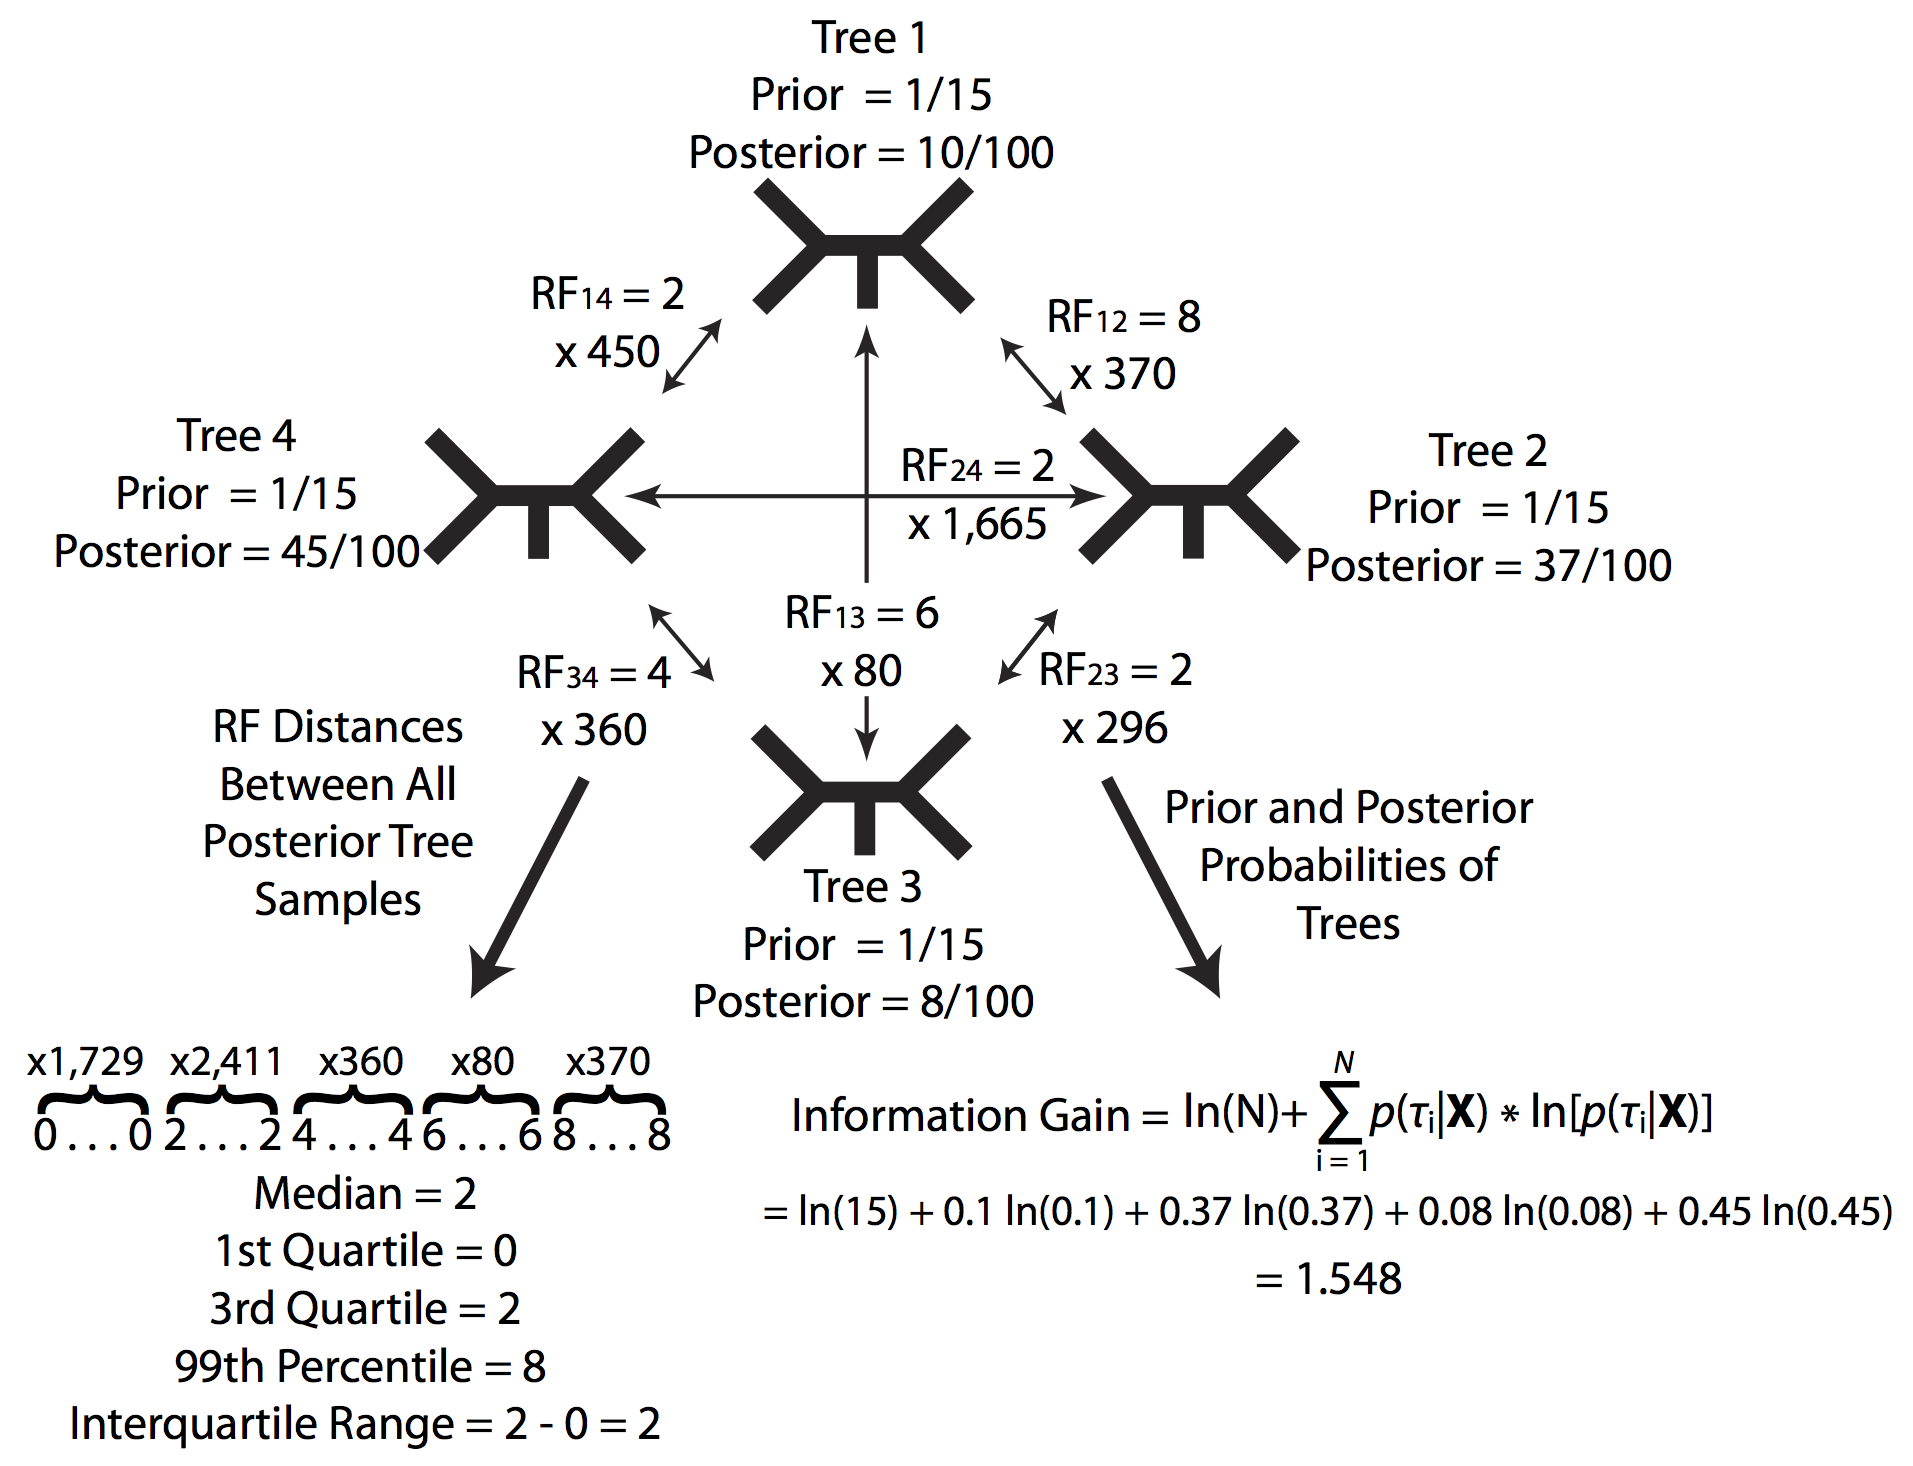
\includegraphics[width=\textwidth,angle=0]{figures/teststats.png}
\caption{\small A diagram showing an example of calculating the inference-based test statistics for a single posterior predictive simulation \citep{Brown2014-mb}.
\label{"Figure 2"}}
\end{figure}
\end{centering}

There are functions built-in to \Revbayes to calculate these values for you. Here are some examples
from the \textbf{PosteriorPredictive\_TreeSummary.Rev} script: 

{\tt \begin{snugshade*}
\begin{lstlisting}
rf_dists <- sim_tree_trace.computePairwiseRFDistances(credibleTreeSetSize=1.0,verbose=FALSE)
mean_rf <- mean(rf_dists)
quantile\_N = quantile(rf_dists, N)
\end{lstlisting}
\end{snugshade*}}

\smallbreak
For posterior predictive simulation, statistical entropy is analogous to the uncertainty associated 
with sampling from the prior or posterior. As the data provide more information and the posterior probabilities of various topologies
become increasingly uneven, entropy decreases causing the difference between the entropy of the prior and the posterior to increase.
Assuming a uniform prior on topologies, the change in entropy can be calculated as:


\begin{equation *} 
$$T_e(X,M_c)=ln[B(N)]+\sum_{i=1}^{B(N)} p(\tau_i|X)ln[p(\tau_i|X)]$$
\end{equation}

The statistical entropy is calculated with the following function call: 

{\tt \begin{snugshade*}
\begin{lstlisting}
sim_tree_trace = readTreeTrace(inFileName,treetype="non-clock")
entropy <- sim_tree_trace.computeEntropy(credibleTreeSetSize=1.0,verbose=FALSE)
\end{lstlisting}
\end{snugshade*}}

These same statistics are calculated for both the posterior distributions from the simulated datasets
and the posterior distribution from the empirical dataset.

Once we have the test statistics calculated for the simulated and empirical posterior distributions, 
we can compare the simulated to the empirical to get a goodness-of-fit. One simple way to do this is to calculate a posterior 
predictive \textit{P}\-value for each of the test statistics of interest. This is done in the \textbf{full\_analysis\_JC.Rev} with the following lines :

{\tt \begin{snugshade*}
\begin{lstlisting}
## CALCULATE INFERENCE P-VALUES
analysis_name = "pps_example"
model_name = "JC"
emp_pps_file = "results_" + model_name + "/empirical_inference_" + analysis_name + ".csv"
sim_pps_file = "results_" + model_name + "/simulated_inference_" + analysis_name + ".csv"
outfileName = "results_" + model_name + "/inference_pvalues_effectsizes_" + analysis_name + ".csv"
statID = v("", "mean_rf", "quantile25", "quantile50", "quantile75", "quantile99", "quantile999", "mean_tl", "var_tl", "entropy")
source("scripts/PosteriorPredictive_PValues.Rev")
clear()
\end{lstlisting}
\end{snugshade*}}

The 3 posterior predictive \textit{P}\-values currently
calculated by \Revbayes are: 

\begin{itemize}
\item Lower 1-tailed 
\item Upper 1-tailed
\item 2-tailed
\end{itemize}

The posterior predictive \textit{P}\-value for a lower one-tailed test is the proportion of samples in the distribution
where the value is less than or equal to the observed value, calculated as:

\begin{equation *} 
$$p_l=p(T(X_r_e_p)\leqslant T(X)|(X)$$
\end{equation}

The posterior predictive \textit{P}\-value for a lower one-tailed test is the proportion of samples in the distribution
where the value is greater than or equal to the observed value, calculated as:

\begin{equation *} 
$$p_u=p(T(X_r_e_p)\geqslant T(X)|(X)$$
\end{equation *}

and the two-tailed posterior predictive \textit{P}\-value is simply twice the minimum of the corresponding one-tailed tests
calculated as:

\begin{equation *} 
$$p_2=2min(p_l,p_u)$$
\end{equation}

Let's take a look at the \textbf{PosteriorPredictive\_PValues.Rev} script to get a better idea of what is 
happening.

Using the equations outlined above, this script reads in the simulated and empirical data we just calculated, and calls a few simple functions: 

{\tt \begin{snugshade*}
\begin{lstlisting}
## Calculate and return a vector of lower, equal, and upper pvalues for a given test statistic
p_values <- posteriorPredictiveProbability(numbers, empValue)

## 1-tailed
lower_p_value <- p_values[1] 
equal_p_value <- p_values[2] 
upper_p_value <- p_values[3] 

## mid-point
midpoint_p_value = lower_p_value + 0.5*equal_p_value

## 2-tailed
two_tail_p_value = 2 * (min(v(lower_p_value, upper_p_value)))
\end{lstlisting}
\end{snugshade*}}

these snippets calculate the various p-values of interest to serve as our goodness-of-fit test. 


Another way that you can calculate the magnitude of the discrepancy between the empirical and PP datasets is by
calculating the effect size of each test statistic. Effect sizes are useful in quantifying the magnitude of the difference between the 
empirical value and the distribution of posterior predictive values. The test statistic effect size can be calculated by taking the 
absolute value of the difference between the median posterior predictive value and the empirical value divided by 
the standard deviation of the posterior predictive distribution \citep{Doyle2015-qb}. Effect sizes are calculated automatically for the inference based test statistics in the P\sur{3} analysis. The effect sizes for each test statistics are stored in the same output file as the \textit{P}\-values. 

{\tt \begin{snugshade*}
\begin{lstlisting}
effect_size = abs((m - empValue) / stdev(numbers))
\end{lstlisting}
\end{snugshade*}}


calculates the effect size of a given test statistic. 



Let's go ahead and calculate the inference-based test statistics now. At your \RevBayes prompt, type the 
following commands: 

{\tt \begin{Snugshade}[184,207,236]
\begin{lstlisting}  
analysis_name = "pps_example"
model_name = "JC"
emp_pps_file = "results_" + model_name + "/empirical_inference_" + analysis_name + ".csv"
sim_pps_file = "results_" + model_name + "/simulated_inference_" + analysis_name + ".csv"
outfileName = "results_" + model_name + "/inference_pvalues_effectsizes_" + analysis_name + ".csv"
statID = v("", "mean_rf", "quantile25", "quantile50", "quantile75", "quantile99", "quantile999", "mean_tl", "var_tl", "entropy")
source("scripts/PosteriorPredictive_PValues.Rev")
clear()
\end{lstlisting}
\end{Snugshade}}

Depending on your computer and how densely you sampled the posterior this process can take from a few minutes to a few hours. If you followed along our tutorial suggestions, this step should take less than 30 minutes to complete. 

Once execution of the script is complete, you should see a new directory, names \textbf{results\_JC}. In this folder there should be 3 files. Each of these is a simple tab-delimited (TSV) file containing the test statistic calculation output.

\begin{itemize}
\item empirical\_pps\_example.tsv
\item pps\_example.tsv
\item pvalues\_pps\_example.tsv
\end{itemize}

If you have these 3 files, and there are results in them, you can go ahead and clear() \RevBayes.

{\tt \begin{Snugshade}[184,207,236]
\begin{lstlisting}  
clear()
\end{lstlisting}
\end{Snugshade}}

You can get an estimate of how the model performed by examining the \textit{P}\-values in the 
\textbf{inference\_pvalues\_effectsizes\_pps\_example.csv} and \textbf{data\_pvalues\_effectsizes\_pps\_example.csv} files. In this example, a quick view shows us that most of the statistics show a value less than 0.05. This leads to a rejection of the model, suggesting 
that the model employed is not a good fit for the data. This is the result we expected given we chose a very 
simplistic model (JC) that would likely be a poor fit for our data. However, it's a good example 
of the sensitivity of this method, showing how relatively short runtimes and a low number of generations will 
still detect poor fit. 


\subsection{Additional Exercises}

Included in the \textbf{scripts} folder is a second model script called \textbf{GTR\_Model.Rev}. 
As a personal exercise and a good test case, take some time now, and run the same analysis, substituting
the \textbf{GTR\_Model.Rev} model script for the \textbf{JC\_Model.Rev} script we used in the earlier example.
This is a good chance to run the full anlaysis using the single-run script by calling \textbf{full\_analysis\_GTR.Rev} script.  
You should get different results, this is an excellent chance to explore the results and think about what
they suggest about the fit of the specified model to the dataset. 

Once you have made the necessary changes, you should be able to execute the full PPS analysis by typing:

{\tt \begin{Snugshade}[184,207,236]
\begin{lstlisting}  
source("scripts/full_analysis.Rev")
\end{lstlisting}
\end{Snugshade}}

\newpage
\subsubsection{Additional Exercises}
\textbf{Some Questions to Keep in Mind:}
\begin{itemize}
  \item Do you find the goodness-of-fit results to suggest that the GTR or JC model is a better fit for our data? 
  \item Which test statistics seem to show the strongest effect from the use of a poorly fitting model?
  \item Other than \textit{P}\-values, what other ways might you explore the test statistic distributions to identify poor fit?
\end{itemize}

\begin{figure}[h]
\centering
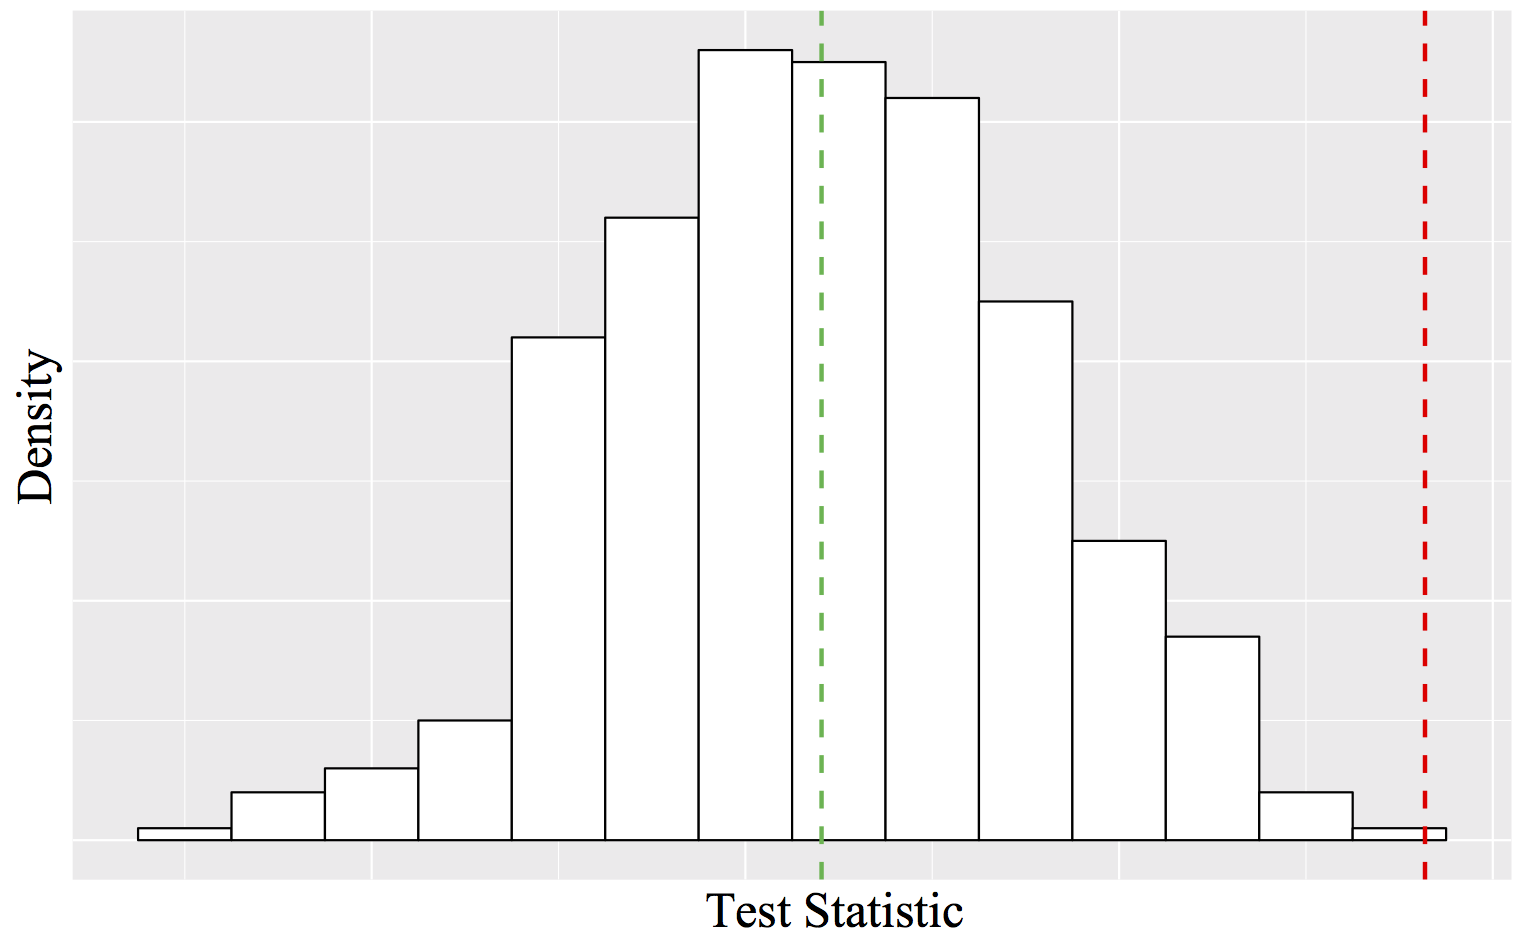
\includegraphics[width=\textwidth,angle=0]{figures/dist.png}
\caption{\small A cartoon showing a hypothesized distribution of a posterior predictive test statistic. The red
line represents the empirical value in a poorly fitting model, the green line represents the empirical value in
a reasonable model. Exploring the fit of a model to the data in a graphical way can often be the easiest way to 
identify a model with a poor fit. \label{"Figure 3"}}
\end{figure}
\end{centering}

\newpage
\section{For your consideration...}
In this tutorial you have learned how to use \RevBayes to assess the fit of a substitution model 
to a given sequence alignment. As you have discovered, the observed data should be plausible under 
the posterior predictive simulation if the model is reasonable. In phylogenetic analyses we choose a model, which explicitly assumes 
that it provides an reasonable explanation of the evolutionary process that generated our data. However, 
just because a model may be the 'best' model available, does not mean it is an appropriate model for the data. 
This distinction becomes both more critical and less obvious in modern analyses, where the 
number of genes often number in the thousands. Posterior predictive simulation in \RevBayes, allows you
to easily check model fit for a large number of genes by using global summaries to check the posterior 
predictive distributions with a comfortable goodness-of-fit style framework. 

\subsection{Batch Processing of Large Datasets}
The process described above is for a single gene or alignment. However, batch processing a large number of genes
with this method is a relatively straight forward process. 

\RevBayes has built in support for MPI so running \RevBayes on more than a single processor, or on a cluster is 
as easy as calling it with openmpi. 

For example:
{\tt \begin{snugshade*}
\begin{lstlisting}
mpirun -np 16 rb-mpi scripts/full_analysis.Rev
\end{lstlisting}
\end{snugshade*}}
would run the entire posterior predictive simulation analysis on a single dataset using 16 processors
instead of a single processor. Use of the MPI version of \RevBayes will speed up the process dramatically.

Setting up the \textbf{full\_analysis.Rev} script to cycle through a large number of alignments is relatively
simple as well. One easy way is to provide a list of the data file names, and to loop through 
them. As an example:

{\tt \begin{snugshade*}
\begin{lstlisting} 
data_file_list = "data_file_list.txt" 
data_file_list <- readDiscreteCharacterData(data_file_list)
file_count = 0

for (n in 1:data_file_list.size()) {

FULL_ANALYSIS SCRIPT GOES HERE

file_count = file_count + 1
}
\end{lstlisting}
\end{snugshade*}}

Then, anywhere in the full\_analysis portion of the script that the lines
{\tt \begin{snugshade*}
\begin{lstlisting} 
inFile = "data/8taxa_500chars_GTR.nex"
analysis_name = "pps_example"
\end{lstlisting}
\end{snugshade*}}
appear, you would replace them with something along the lines of: 
{\tt \begin{snugshade*}
\begin{lstlisting} 
inFile = n
analysis_name = "pps_example_" + file_count
\end{lstlisting}
\end{snugshade*}}

This should loop through all of the data files in the list provided, and run the full posterior predictive
simulation analysis on each file. Using a method like this, and combining it with the MPI call above, you can scale
this process up to multiple genes and spread the computational time across several cores to speed it up. 

\bigskip
\bibliographystyle{sysbio}
\bibliography{pps}